\documentclass{beamer}
\usepackage[utf8]{inputenc}
\usepackage[english,french]{babel}
\usepackage{tabularx}
\usepackage{graphicx}
\usepackage{epstopdf}

\usetheme{Antibes}
\title[CryptoSMS]{CryptoSMS\\Text message encryption for Android}
\author{David Brazdil}
\institute{University of Cambridge}
\date{September 15, 2011}

% TEXT CONSTANTS
\newcommand{\txtFacts}{Facts}
\newcommand{\txtStorageFile}{Storage file}
\newcommand{\txtTextCompression}{Text compression}
\newcommand{\txtTextMessaging}{Text messaging}

% MARGIN AND PADDING IN TABLES
\renewcommand*\arraystretch{1.5}
\newcommand{\verticalspace}{\vspace{10pt}}

\begin{document}
\newcolumntype{L}{>{\raggedright\arraybackslash}X}%

\begin{frame}
	\titlepage
\end{frame}

% FACTS

\begin{frame}{\txtFacts}{Attacker}
	\begin{itemize}
		\pause \item{Can read and manipulate everything you send}
		\pause \item{Can gain physical access to your handset}
		\pause \item{Can install a malicious application on your phone}
	\end{itemize}
\end{frame}

% DEMO

% TEXT MESSAGING

\begin{frame}{\txtTextMessaging}{Data structure}

	\begin{block}{First part}
		\verticalspace
		\begin{tabularx}{\textwidth}{ |l|l|l|l|L| }
			\hline
			type1, id   & count   & IV   & HMAC & data \\
			2 B         & 1 B     & 16 B & 32 B & 84 B  \\
			\hline
		\end{tabularx}
	\end{block}

	\begin{block}{Other parts}
		\verticalspace
		\begin{tabularx}{\textwidth}{ |l|l|L| }
			\hline
			type2, id  & index   & data \\
			2 B    & 1 B  & 130 B  \\
			\hline
		\end{tabularx}
	\end{block}
\end{frame}

\begin{frame}{\txtTextMessaging}{\txtTextCompression}
	\begin{exampleblock}{French}
		\foreignlanguage{french}{Salut Pierre, {\c c}a va? Je suis désolé, mais je ne serai pas là à cinq heures, parce que je suis malade. Je suis libre ce lundi et toi? Quand tu as quelques problèmes, appelles-moi. J'espère que tout sera ok.}

		\verticalspace
		\centering
		\begin{tabular}{ |c|c|c|c| }
			\hline
			UTF-16 & UTF-16 + DEFLATE & UTF-8 & UTF-8 + DEFLATE \\
			\hline
			412 B & 210 B & 212 B & 164 B \\
			\hline
		\end{tabular}
	\end{exampleblock}
\end{frame}

% KEY NEGOTIATION

\begin{frame}
  
   \begin{alertblock}{This is an Alert block}
   This is an important alert
   \end{alertblock}
 
   \begin{exampleblock}{This is an Example block}
   This is an example 
   \end{exampleblock}
 
\end{frame}

% STORAGE FILE

\begin{frame}{\txtStorageFile}{Internal structure}

	\centering
	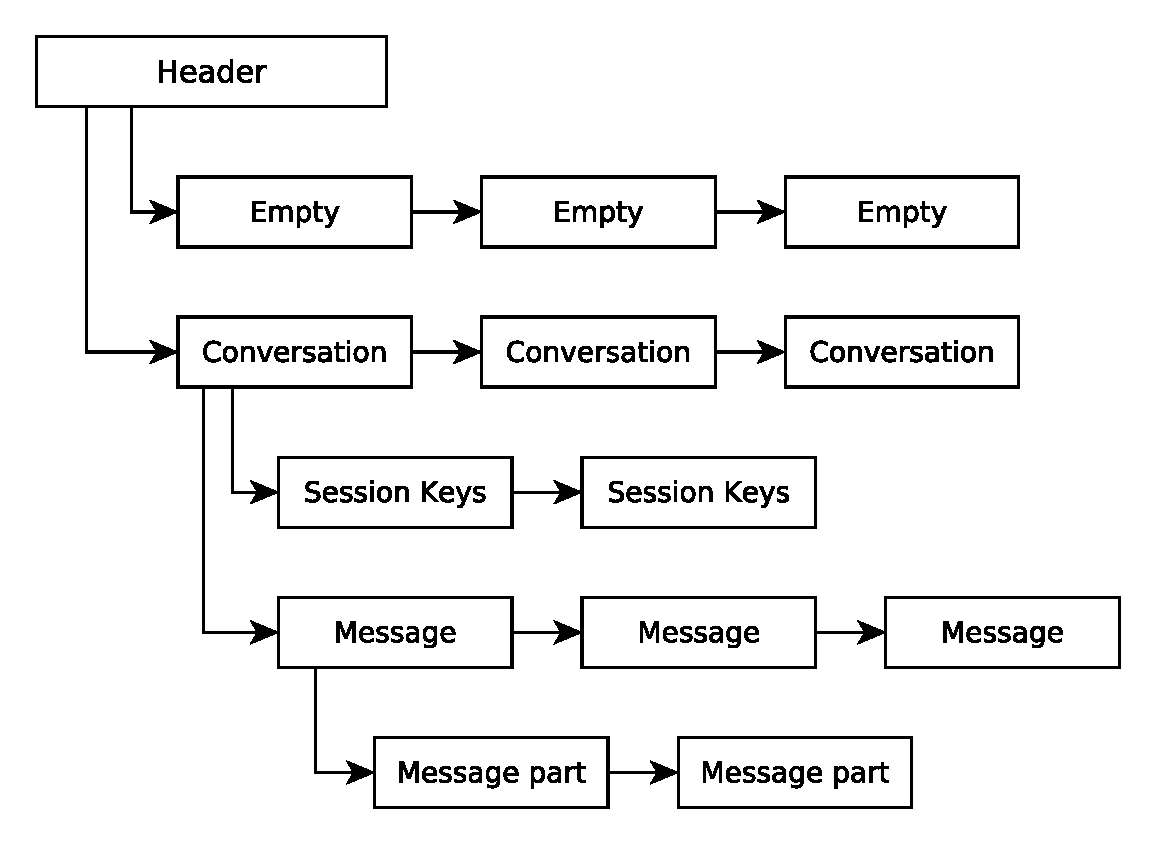
\includegraphics[width=0.8\textwidth]{storage_file}
\end{frame}

\begin{frame}{\txtStorageFile}{From the outside}

	\begin{tabularx}{\textwidth}{ |l|l|L| }
		\hline
		IV & HMAC & Encrypted header \\
		\hline
		IV & HMAC & Encrypted entry 1 \\
		\hline
		IV & HMAC & Encrypted entry 2 \\
		\hline
		IV & HMAC & Encrypted entry 3 \\
		\hline
		IV & HMAC & Encrypted entry 4 \\
		\hline
		IV & HMAC & Encrypted entry 5 \\
		\hline
		IV & HMAC & Encrypted entry 6 \\
		\hline
		IV & HMAC & Encrypted entry 7 \\
		\hline
	\end{tabularx}

	\centering
	$\vdots$ \\
\end{frame}

% PKI COOPERATION

% SUMMARY
% create a check list of aims

\end{document}